\section{Overall Description}

\subsection{Product Perspective}

\subsubsection{Scenarios}
\begin{enumerate}
    \item \textbf{Student signs up for a tournament}
    \newline
    Luca, eager to increase his skills in software development, learned of the existence of CodeKataBattle (CKB), a system dedicated to programming tournaments based on CodeKata exercises in which students can compete. Taken by interest, Luke registered on the CKB platform and checked out the tournaments that had not yet started. Having chosen the tournament, Luca registers.  The CKB system presents Luca with a list of available battles within the tournament,  allowing him to select one when the tournament begins. The system notified Luca whenever a new battle was created.


    \item \textbf{Student signs up for a battle}
    \newline
    Pasquale, an experienced Java programming student, is looking for opportunities to expand his skills in different languages. Exploring the list of available challenges on CodeKata, he would like to select a challenge based on Python, a language with which he has less experience. However, to tackle this new challenge with more confidence, he is interested in participating in a group with other students. Next, Pasquale examines the still open battles in which it is possible to participate.
    \newline
    Once enrolled in a specific battle, Pasquale decides to invite his friend Marco to join him in tackling this challenge. Once the battle begins, the CodeKataBattle system sends Pasquale the link to the GitHub repository containing the CodeKata and the instructions necessary to configure the platform to receive notifications regarding each commit and push made by the team.
    
  
    
    \item \textbf{The team works on the project}
    \newline
    Team members, consisting of a group of friends, start collaborating on the project. To make sure everything gets done right, they create a fork of the GitHub repository and, using GitHub Actions, set up an automated workflow to inform the CodeKataBattle (CKB) platform whenever a commit is made to the main branch of their repository.
    \newline
    Once the first push is made, , the CKB pulls the source uploaded by the team to GitHub, and assigns a score from 0 to 100 based on the number of test cases that pass, the time difference between the battle registration deadline and the last commit made, and uses an external tool to do static analysis and evaluate the source on certain aspects entered at battle creation time by the educated.
    \newline
    After scoring, the system proceeds to update the current ranking. This procedure allows the team to access information about the current position occupied within the ranking.
    \newline
    After the final project submission deadline, the CKB platform notifies the team that the final battle ranking is available.


    %manages a tournament life cycle 
    \item \textbf{Educator manages a tournament}
    \newline
    Alessandro, a university lecturer in object-oriented programming, chose to adopt the CKB platform to organise a tournament. This initiative allows the students on his course to compete against individuals outside the academic context, giving them a broader opportunity for challenge and comparison.
    \newline
    Alexander creates the tournament by setting a tournament entry deadline, and with the goal of enriching the variety of battles, he invited his fellow educators to collaborate in creating the battles. Once created, the platform will inform all participants of the new competition.
    \newline
    Once Alexander considers the number of battles that occurred in the context of the tournament he organized to be satisfactory, and once these have ended, he makes the decision to end the tournament. To this end, the system proceeds to notify all students participating in the tournament, of the available of the final ranking.




    \item \textbf{Educator organises a battle}
    \newline
    Gianluca, an expert in C++ programming, decided to organise a battle concerning a specific CodeKata that aroused particular interest. The CKB platform requested him to provide all the necessary specifications to set up the battle, including CodeKata upload, the deadline for registrations, the minimum and maximum limits of students per group and the deadline for the delivery of projects, and he choose maintainability and reliability as evaluation aspects.
    \newline
    In addition, Gianluca chose to participate in the final evaluation of the projects submitted in the battle.
    \newline
    During the course of the battle, the system provides Gianluca with the current score and ranking of the teams participating in the battle. At the end of the battle, Gianluca examines the final sources of each team and evaluates them personally.
    


\end{enumerate}


\vspace{0.5\baselineskip}
\subsubsection{Domain class diagram}
In Fig(\ref{fig_DomainClassDiagram}) is represented the Domain Class Diagram related to the CKB. It contains all the domain elements in which the system operates and interacts between elements. In the following we will describe the most relevant parts of the diagram: 
\begin{itemize}
    \item There are two types of users: Student and Educator. They have things in common such as first name, last name and email.
    
    \item Only one educator is allowed to create a tournament; however, multiple educators may participate in that tournament. Each tournament must include at least one battle.
    
    \item In the context of the battle, one or more teams may participate, each consisting of at least one student who is involved in the tournament in which this battle takes place .
    
    \item Each team has a GitHub repository in which the last project actually uploaded (pushed) is stored, along with the direct link of the GitHub repository and the score assigned by the system for each push. The mentioned repository hosts the CodeKata related to the battle in which the team participated. Each team may be subject to a score by a specific one, on the final project submitted.


\end{itemize}

\begin{figure}[h]
    \centering
    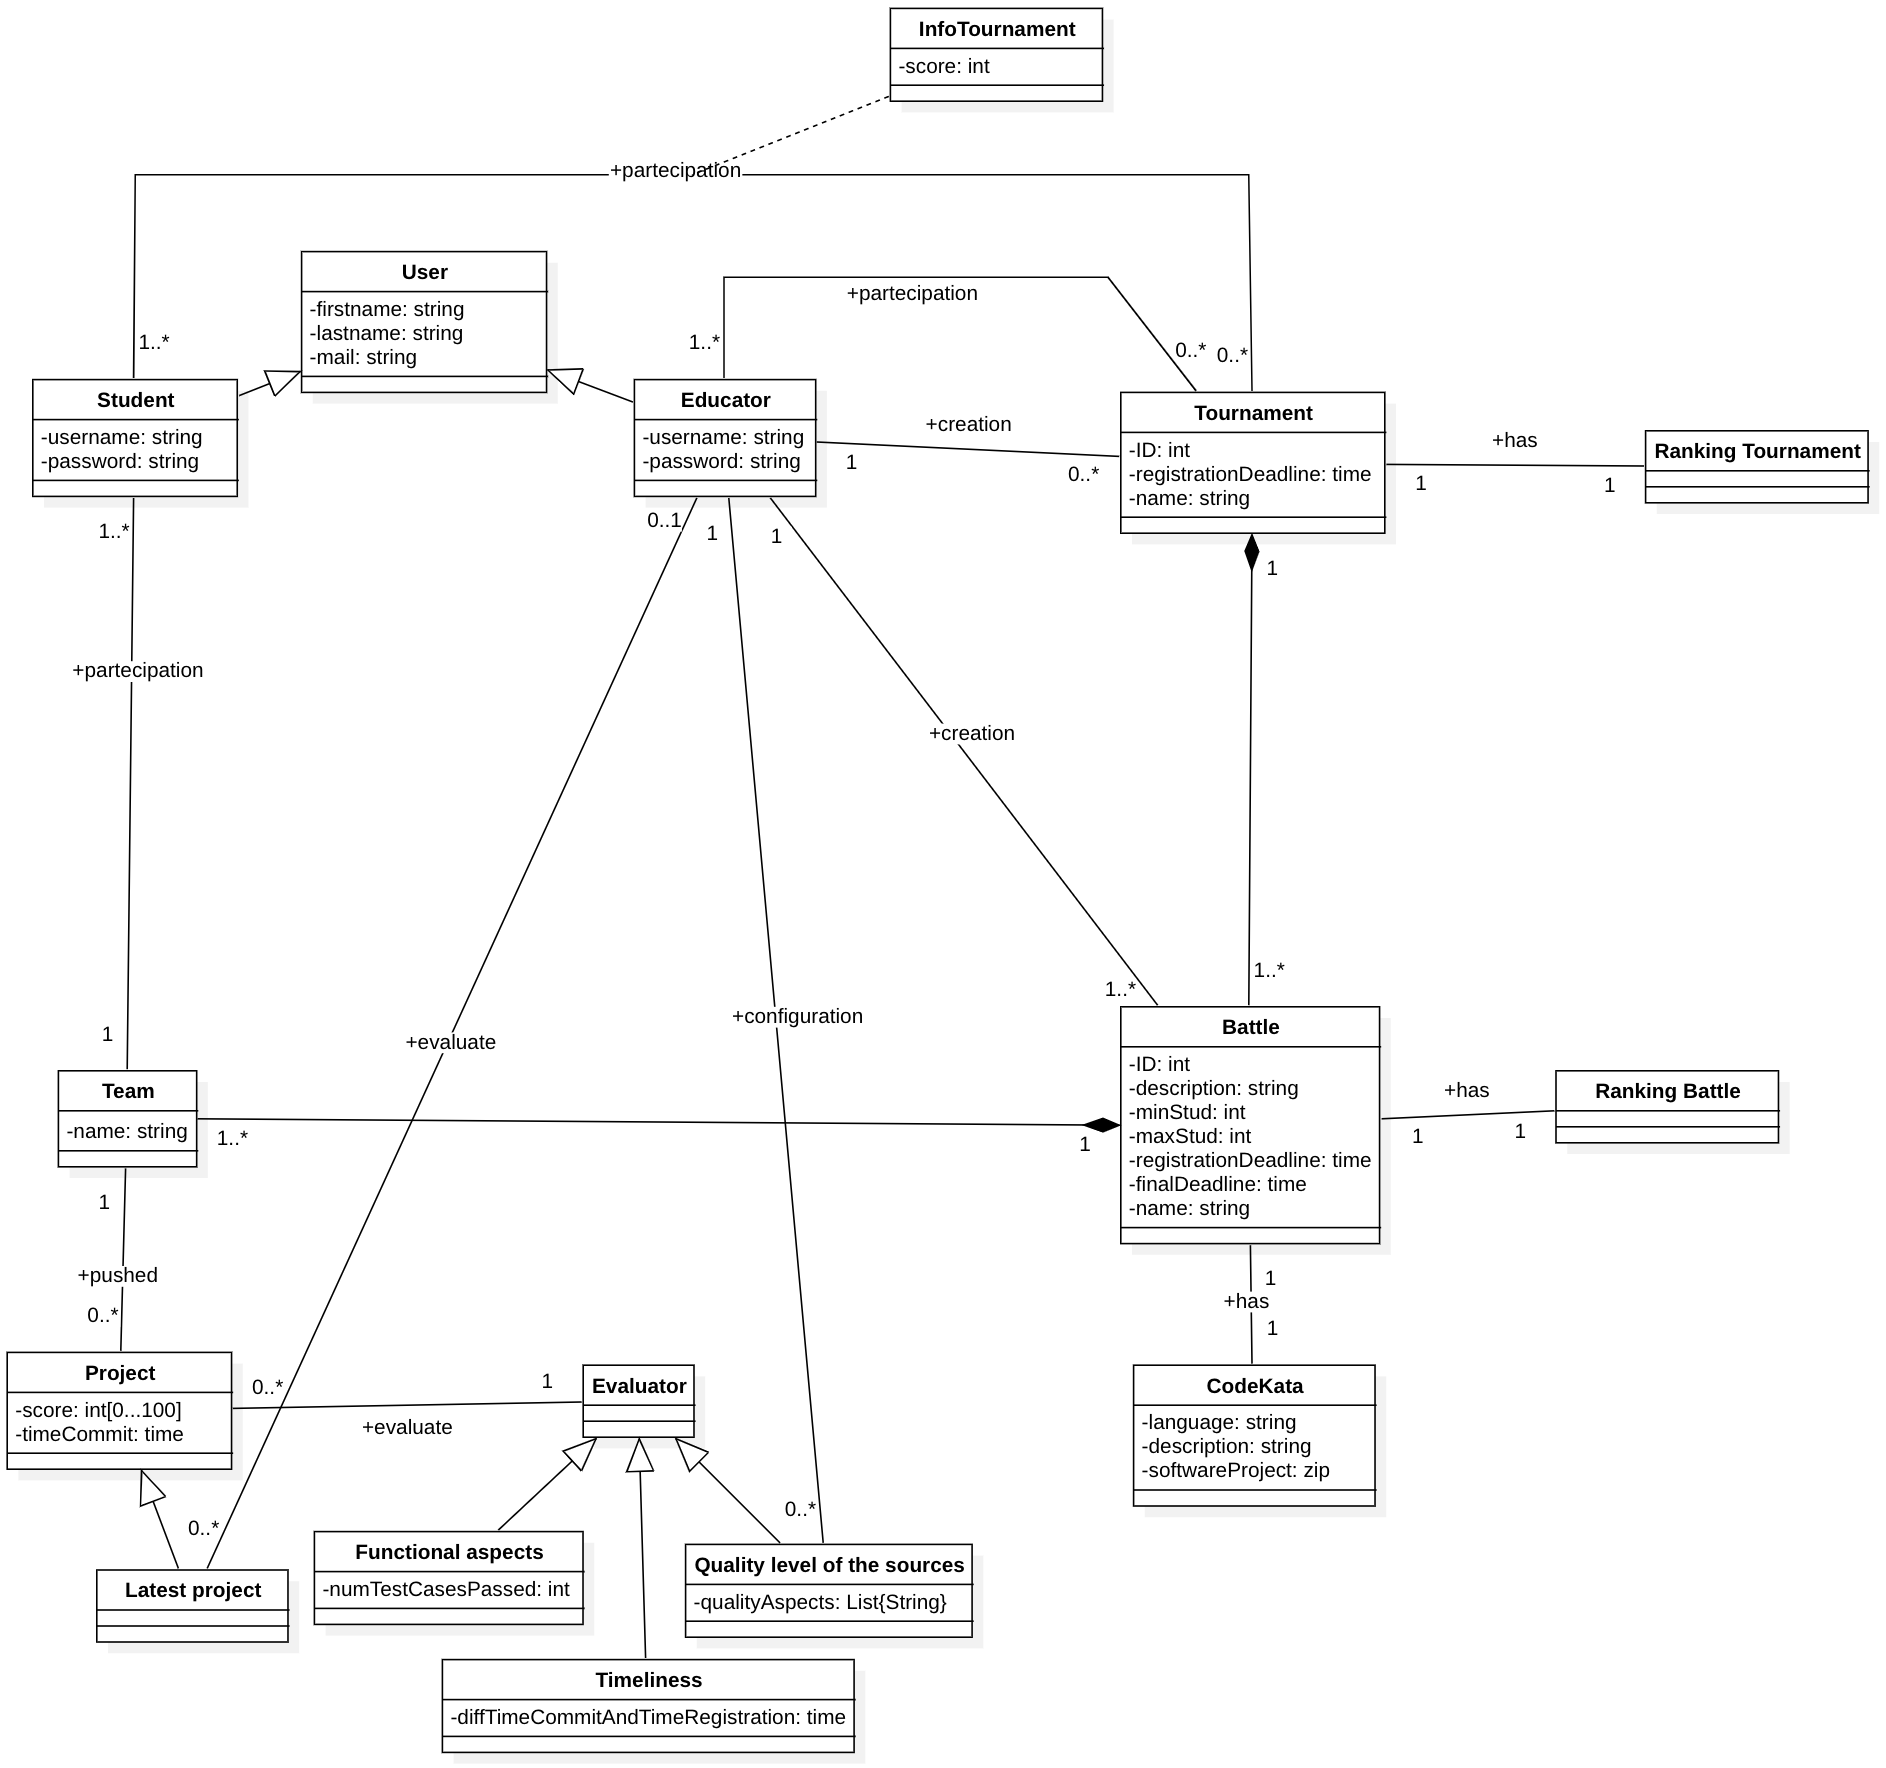
\includegraphics[scale=0.55]{images/ClassDiagramCKB.png} 
    \caption{Domain Class Diagram}
    \label{fig_DomainClassDiagram}
\end{figure}

\clearpage
\subsubsection{Statecharts}
In this section, the state diagrams for Tournament, Team and Battle were examined.
\newline
These diagrams offer a representation of the life cycle of an object of a specific class, highlighting the states through which the object transits during its life cycle and the conditions that determine these transitions from one state to another.

\vspace{1\baselineskip}

\textbf{Status of Tournament}

\counterwithin{figure}{subsection}
\begin{figure}[h]
    \centering
    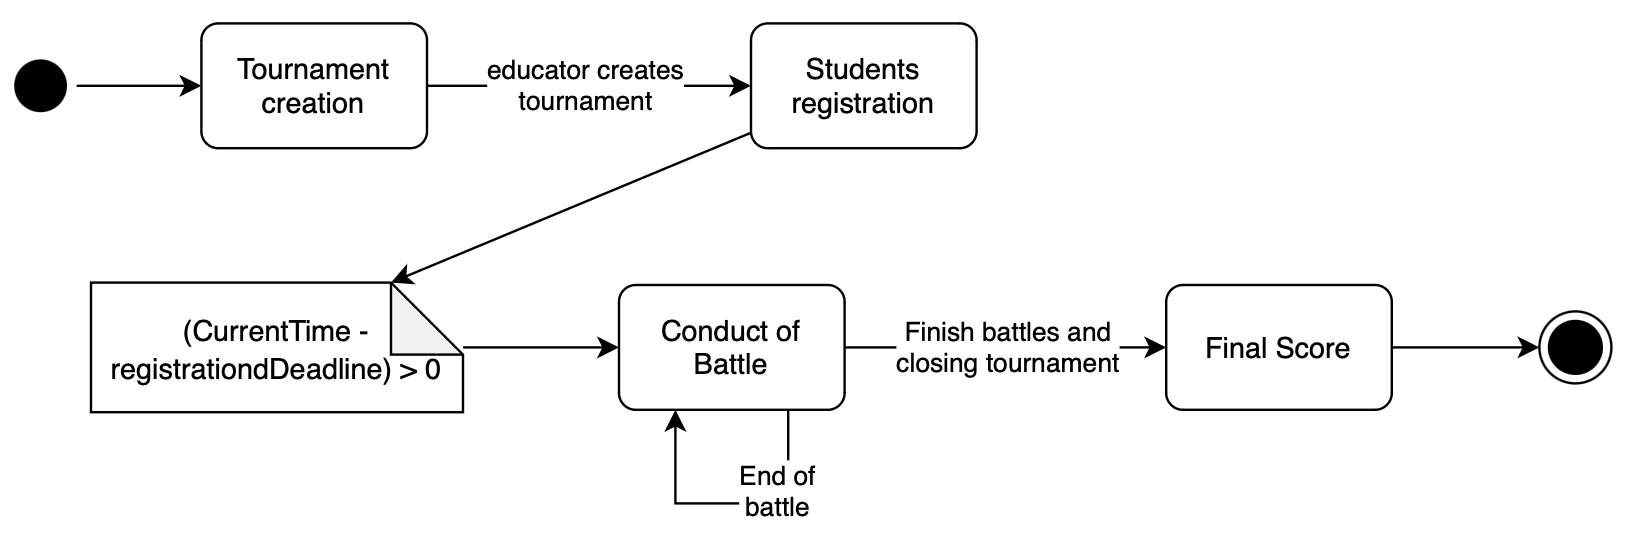
\includegraphics[scale=0.4]{images/Statecharts/TournamentCreation.png} 
    \caption{Tournament status}
    \label{fig_TournamentCreation}
\end{figure}

Figure \ref{fig_TournamentCreation} presents the state diagram describing the life cycle of an instance of the tournament class.
\newline
The process begins in the initial state, called \textbf{\textit{Tournament Creation}}, the phase in which an educator wants to start a tournament. During this phase, the educator may invite other colleagues to participate in the creation of battles within the tournament.
\newline
After the creation of the tournament by the educator, the system moves to \textbf{\textit{Student Registration}} status, allowing students to register for the tournament.
\newline
Once the deadline to register for the tournament has passed,calculated by the difference between the currentTime and the registrationDeadline, the tournament begins, proceeding in the \textbf{\textit{Conduct of Battle}}. In this state, the educators manage the battles they have created. At the end of each battle, the participants' scores are updated and notified.
\newline
Once all battles within the tournament have been concluded and the educator responsible for the tournament decides to close the event, the process transitions into the \textbf{\textit{Final Score}} state. In this state, the ranking of the tournament participants is updated and each participant is notified of the final results of the tournament.



\vspace{1.5\baselineskip}
\textbf{Status of a Team}

\begin{figure}[h]
    \centering
    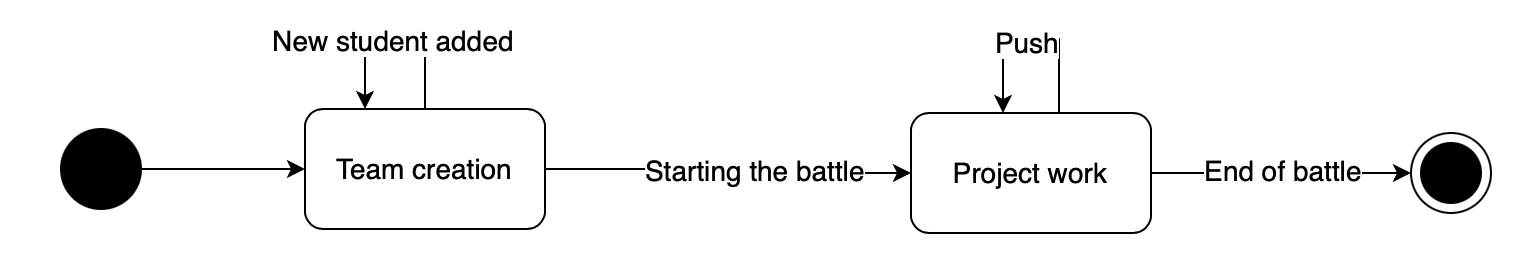
\includegraphics[scale=0.5]{images/Statecharts/TeamStatus.png} 
    \caption{Team Status}
    \label{fig_TeamStatus}
\end{figure}

The figure \ref{fig_TeamStatus} presents the statechart describing the status of a team within a battle context.
\newline
The process begins in its initial state, called \textbf{\textit{Team Creation}}, in which a student participating in a battle forms a team with other students by inviting them, respecting the specific constraints of the battle they are joining.
\newline
After the start of the battle, the team enters the \textbf{\textit{Project Work}} state. In this phase, team members work on the Code Kata associated with the battle, making regular pushes to GitHub and receiving feedback.
\newline
The process finally reaches its terminal state at the end of the battle.


\vspace{1.5\baselineskip}
\textbf{Status of Battle}

\begin{figure}[h]
    \centering
    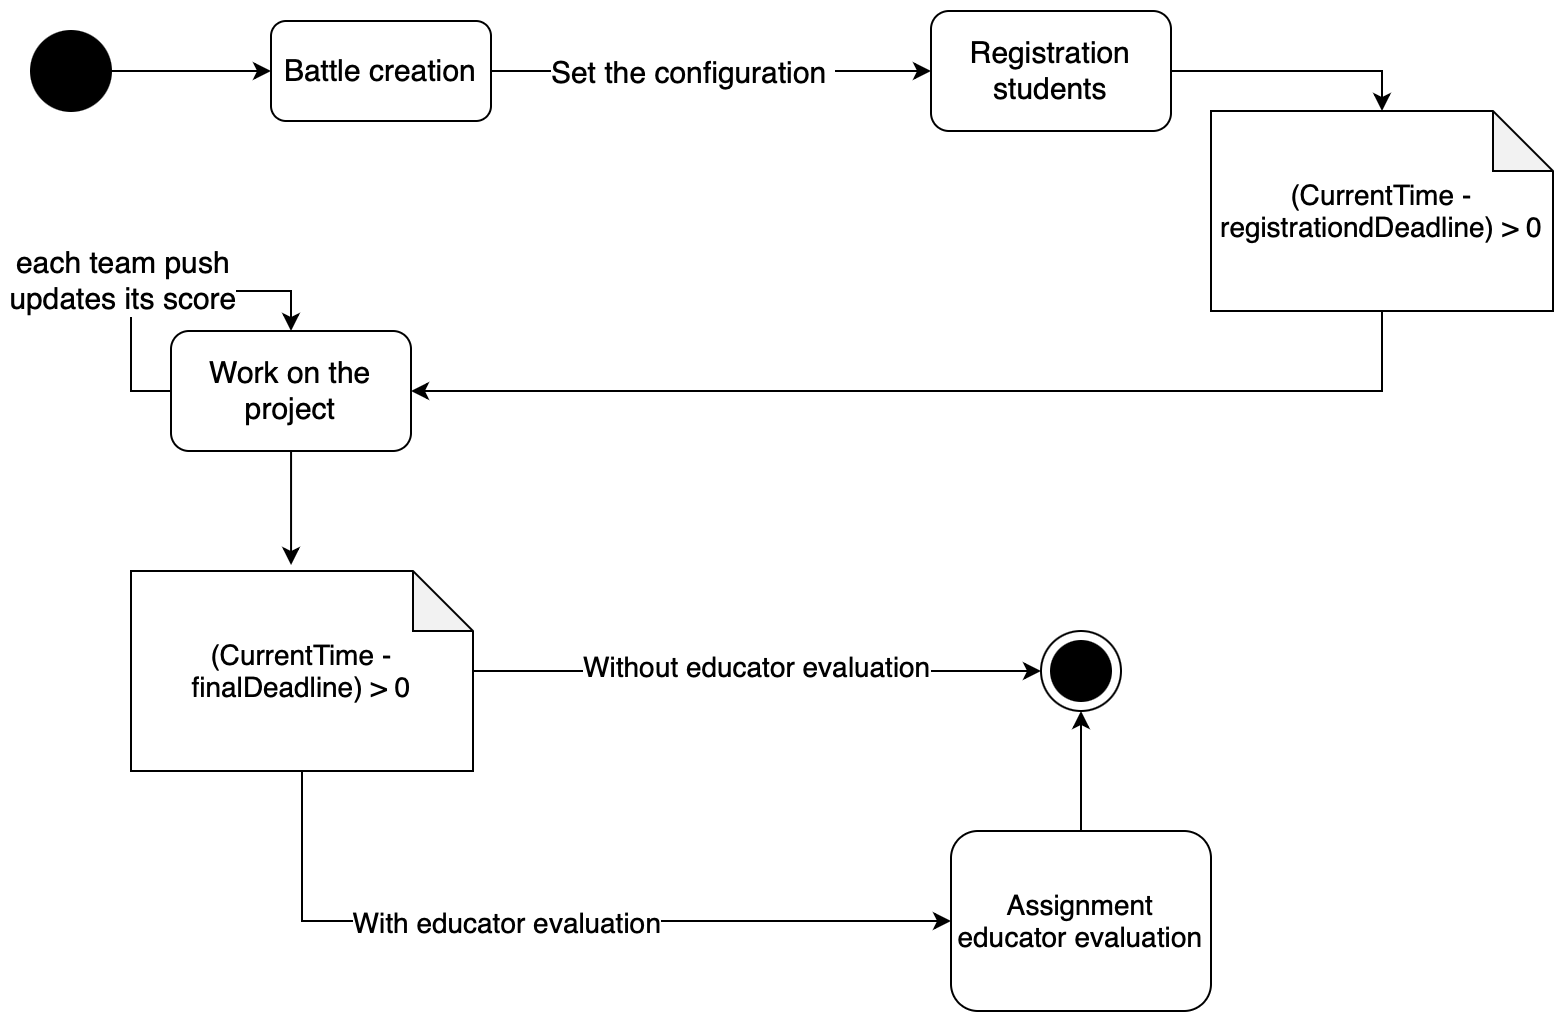
\includegraphics[scale=0.4]{images/Statecharts/BattleCreation.png} 
    \caption{Battle Creation}
    \label{fig_BattleCreation}
\end{figure}

The figure \ref{fig_BattleCreation} illustrates the statechart relating to the procedure of creating a battle by an educator.
\newline
The process begins in the initial state, represented by \textbf{\textit{Battle Creation}}, in which the battle parameters are configured.
\newline
It then transitions into the \textbf{\textit{Registration students}} state, where interested students register and invite other students to form teams to participate in the battle. When the registration deadline is reached, calculated by the difference between the currentTime and the registrationDeadline, the battle starts the operational phase by entering the \textbf{\textit{Work on the Project}} state, during this phase the teams receive the link to the GitHub repository and the instructions to be followed to enable correct operation, after which they start working on the project by pushing on the repository, in this way every push before the deadline, the platform calculates and updates the team score.
\newline
At the expiry of the \textbf{\textit{Final Deadline}}, calculated through the difference between the currentTime and the finalDeadline, if the educator has not made a decision regarding scoring, the process transits to the final state.
\newline
Conversely, if the educator decides to evaluate the final project by assigning a score, the process moves to the \textbf{\textit{Assignment Educator Evaluation}} state. At this stage, the educator proceeds with the scoring of the team, finally leading the process to the final state.


\vspace{1.5\baselineskip}
\newpage
\textbf{Status of Student}

\begin{figure}[h]
    \centering
    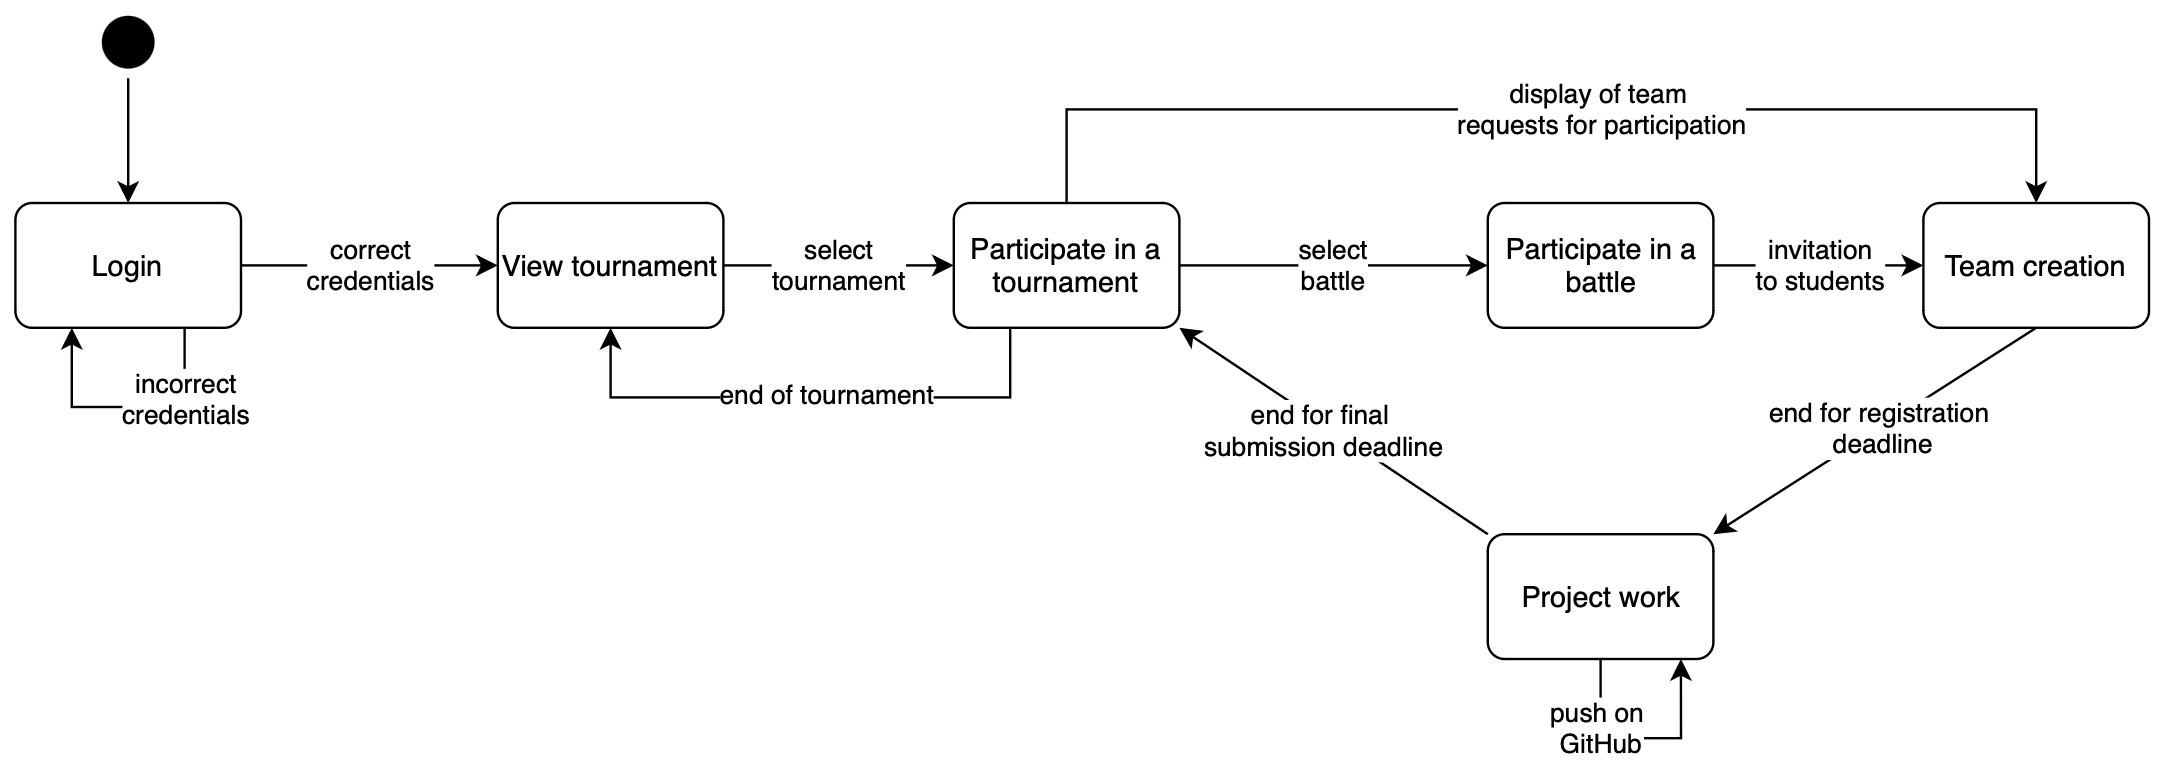
\includegraphics[scale=0.4]{images/Statecharts/StudentStatus.png} 
    \caption{Student status}
    \label{fig_StudentStatus}
\end{figure}

The figure \ref{fig_StudentStatus} illustrates the statechart representing the status of a student within the system.
\newline
The process starts from the initial state \textbf{\textit{Login}}, where the student enters their credentials. If the credentials entered are incorrect, the student remains in that state; otherwise, he moves on to the next state, \textbf{\textit{View tournament}}, where the available tournaments are displayed.
\newline
Once the tournaments are displayed, the student selects the one in which he wishes to participate, passing into the \textbf{\textit{Partecipate in a tournament}} state. In this status, the available battles within the tournament are listed.
In this state, two scenarios can occur:
\begin{itemize}
\item The student selects a specific battle in which he wishes to participate, passing through the \textbf{\textit{Participate in a battle}} status. At this point, the student enrolled in the battle must create a team, inviting other student participants. This transition takes place in the \textbf{\textit{Team creation}} state, where the student enters the team name and invites other participants registered for the tournament.
\item The student receives and accepts a request to participate in a team, moving directly into \textbf{\textit{Team creation}} status.
\end{itemize}

Once the battle registration period has expired, the process moves into the \textbf{\textit{Project work}} state. In this phase, the team works on the received codekata, pushing on GitHub.
\newline
When the final submission phase expires, the student returns to the \textbf{\textit{Participate in a tournament}} state. If the tournament is still running, the student goes through the same status as previously described. However, if the tournament has been closed by the responsible educator, we return to the \textbf{\textit{View tournament}} status, where the available tournaments are shown.






\clearpage

\subsection{Product Functions}

\subsubsection{Sign Up and Login}
This function is accessible to all users.
The registration process for students and educators allows them to register on the platform by entering the required data, including first name, last name, e-mail address, username and password.
\newline
The login function allows users to access the platform using username and password.

\subsubsection{Manage tournaments}
The tournament management function offers educators the possibility of creating tournaments by defining their name and setting a deadline for registrations. They can also invite other educators to participate. In addition, it allows students to register for tournaments and revoke their registration if necessary.
\newline
Each time a tournament is created, the system notifies each platform member. At the end of each battle, the participants' individual scores are updated, representing the sum of the points obtained in the battles completed within the tournament. The ranking of the tournament accordingly is also updated.
\newline
Once all battles have been completed and wishing to close the tournament, the creating educator can proceed to close it. In addition, each user of the CKB platform can view the list of all ongoing tournaments and their respective rankings.

\subsubsection{Participation in tournament }
This functions allows students to sign up for a tournament, and once they sign up and the tournament has started they can see the list of available battles and the tournament ranking with their current score. When the tournament closes, they will be notified that the final ranking is available.

\subsubsection{Manage battle}
The battle management function allows each educator involved to create multiple battles in a tournament.
\newline
When each battle is created, a notification is sent to all students registered for that tournament. At each battle, it is required to upload the CodeKata on which the teams are to focus and to specify the minimum and maximum number of students for each team. In addition, the educator enters a brief description, sets the deadline for registration, the deadline for delivery of the final project and indicates the quality aspects to be sent by the system to a third-party tool for evaluation.
\newline
At the battle deadline, if declared during battle creation, the educator can view the source of the teams and can assign a personal score. Otherwise, the system will close the battle and directly present the final ranking of the battle along with the corresponding score for each team. The system will also inform each student participating in the battle of the availability of the final ranking.

\subsubsection{Participation in battle}
The function allows students to sign up for only one battle at a time, the delivery of invitations for the formation of groups that conform to the limits set by the educator. Once the groups are formed and the battle begins, the system will send each member of each team the link to the main GitHub folder and the instructions to be executed to allow the platform to stay updated on commits and pushes performed by teams. For each push made by the team on its main repository, the system will use 3 parameters: functional aspects, measured in terms of number of test cases that pass out of all test cases,
timeliness, measured in terms of time passed between the registration deadline and the last commit,
quality level of the sources, where the system uses SonarQube to perform static analysis of the source and evaluate it on aspects entered at the time of battle creation by the educator. By assigning a score between 0 and 100. In this way, the team can view the current score and relative position in the ranking with each push.



\clearpage
\subsection{User characteristics}

There are two types of users who interact with the system: Student and Educator.

\subsubsection{Student}
A Student is a person who possesses basic skills in software programming and demonstrates a high level of competence in the use of computing devices. He wishes to increase his skills in software development and uses the CKB system for this purpose.

\vspace{0.5\baselineskip}
\subsubsection{Educator}
An Educator is a person with advanced skills in software development. He is responsible for managing the administrative functions of the system, including the creation of tournaments and battles.


\vspace{1.5\baselineskip}

\subsection{Assumptions, dependencies and constraints}

\subsubsection{Regulatory policies}
The CKB system will ask for user personal information like name, surname and email address. Email addresses won’t be used for commercial purposes. Personal information will be processed in compliance with the GDPR.

\subsubsection{Domain Assumptions}
Below are the assumptions made for the domain. These assumptions are properties and/or conditions that the system takes for granted, mainly because they are outside the control of the system itself, and therefore must be verified to ensure the correct behavior of CodeKataBattle.

\begin{itemize}[left=20pt]
    \setlength{\itemsep}{0pt}
    \setlength{\parskip}{0pt}
    \setlength{\parsep}{0pt}
    \setlength{\partopsep}{0pt}
    \setlength{\topsep}{0pt}
    \item [{[D1]}] Student  must have an internet connection
    \item [{[D2]}] Educator must have an internet connection
    \item [{[D3]}] Educator be a very knowledgeable person in the area of software development
    \item [{[D4]}] Student must have a GitHub account
    \item [{[D5]}] Students who are part of the team when they receive the main GitHub repository must fork it
    \item [{[D6]}] Students who are part of the team must set up an automated workflow through GitHub Actions to inform the platform
    \item [{[D7]}] Students must have all the tools(e.g., IDE) to work on the project
    \item [{[D8]}] Educator must make sure that the CodeKata he intends to upload, we have no errors inside
    \item [{[D9]}] Students participating in a battle are expected to follow a test-first approach
    
\end{itemize}
